\documentclass[hidelinks]{article}
\usepackage{polski}
\usepackage[utf8]{inputenc}

\title{
Geometria Obliczeniowa \\ ~ \\ Dokumentacja projektu \\ ~ \\ Wyszukiwanie najmniejszego okręgu i prostokąta na chmurze punktów\\ ~ \\ 
}
\author{Jakub Stępak}
\date{Grudzień 2016}

\usepackage{graphicx}
\usepackage{amssymb}
\usepackage{gensymb}
\usepackage{listings}
\usepackage{geometry}
\usepackage{hyperref}


\begin{document}

\maketitle

\tableofcontents

\newpage

\section{Opis projektu}

\subsection{Problem}

Zadanie polegało na napisaniu programu, który, na zadanej chmurze punktów, będzie znajdywał:
\begin{itemize}
\item najmniejszy \textbf{okrąg} ją zawierący,
\item prostokąt ją zawierający o minimalnym \textbf{polu},
\item prostokąt ją zawierający o minimalnym \textbf{obwodzie}.
\end{itemize}


\subsection{Wykorzystanie otoczki wypukłej}

Wszystkie rozwiązania będą opierały się o wyznaczoną otoczkę wypukłą zadanej chmury punktów. \\

Program posiada moduł do wyznaczania otoczki wypukłej algorytmem Grahama. Istnieje możliwość łatwego dodania innego algorytmu do wyznaczania otoczki wypukłej i użycie go zamiast dostarczonego.

\newpage

\section{Wyszukiwanie najmniejszego okręgu}

Do znalezienia najmniejszego okręgu używam \textbf{algorytmu Appleta}.

\subsection{Obserwacja}

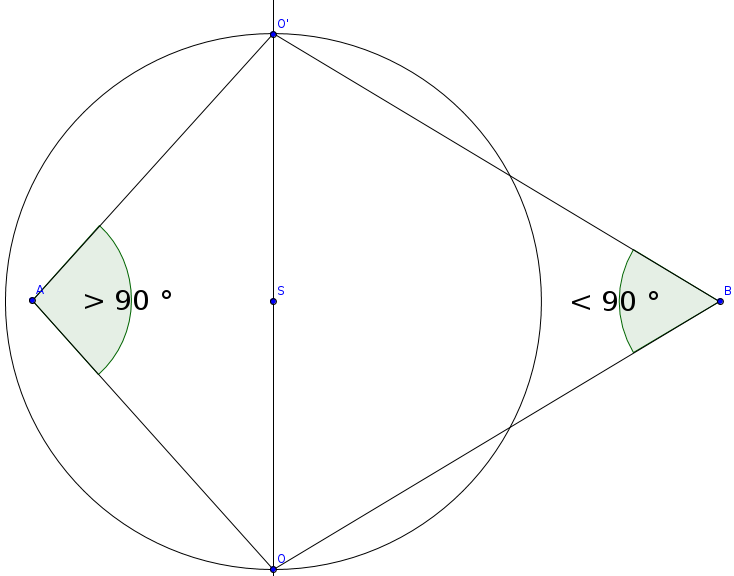
\includegraphics[width=\textwidth]{pics/angles.png}

~ \\

Do zrozumienia działania algorytmu Appleta przydatne będzie zauważenie, że jeśli na średnicy okręgu oprzemy kąt, to:

\begin{itemize}

\item jeśli wierzchołek kąta znajduje się wewnątrz tego okręgu, jego miara jest większa niż $90 \degree $

\item jeśli wierzchołek kąta znajduje się na zewnątrz tego okręgu, jego miara jest mniejsza niż $90 \degree $

\end{itemize}

\newpage

\subsection{Algorytm Appleta - pseudokod}

\begin{enumerate}

\item Wybierzmy dowolną krawędź otoczki $S  = [P_1, P_2]$.

\item Dla każdego wierzchołka $P_0 \neq P_1, P_2$, 
obliczamy $ \measuredangle P_1 P_0 P_2 $. 

\item Najmniejszy znaleziony kąt oznaczmy przez $\alpha$, 
a wierzchołek przy którym występuje przez $V$:

\begin{enumerate}

\item Jeśli $ \alpha > 90 \degree $ to rozwiązaniem jest okrąg opisany na $S$. 
\item  Jeśli $ \alpha < 90 \degree $ sprawdzamy pozostałe 
kąty $ \triangle P_1 V P_2 $:

\begin{enumerate}
\item  Jeśli żaden nie jest rozwarty, to rozwiązaniem 
jest okrąg opisany na $ \triangle P_1 V P_2 $.

\item Jeśli któryś z kątów jest rozwarty, krawędź naprzeciwko niego
staje się nowym $S$. Wracamy do punktu 2.

\end{enumerate}

\end{enumerate}

\end{enumerate}

\subsection{Algorytm Appleta - implementacja}

Na kolejnej stronie znajduje się listing metody $run$ w klasie $Applet$ implementującej algorytm Appleta.

\newgeometry{margin=2cm}
Implementacja algorytmu Appleta:
\begin{center}
\lstinputlisting[language=Python,frame=single,linewidth=1\textwidth]{sourcecodes/applet.py}
\end{center}

\restoregeometry


\subsection{Wynik}
Przykładowy wynik działania programu: \\ ~ \\

\begin{center}
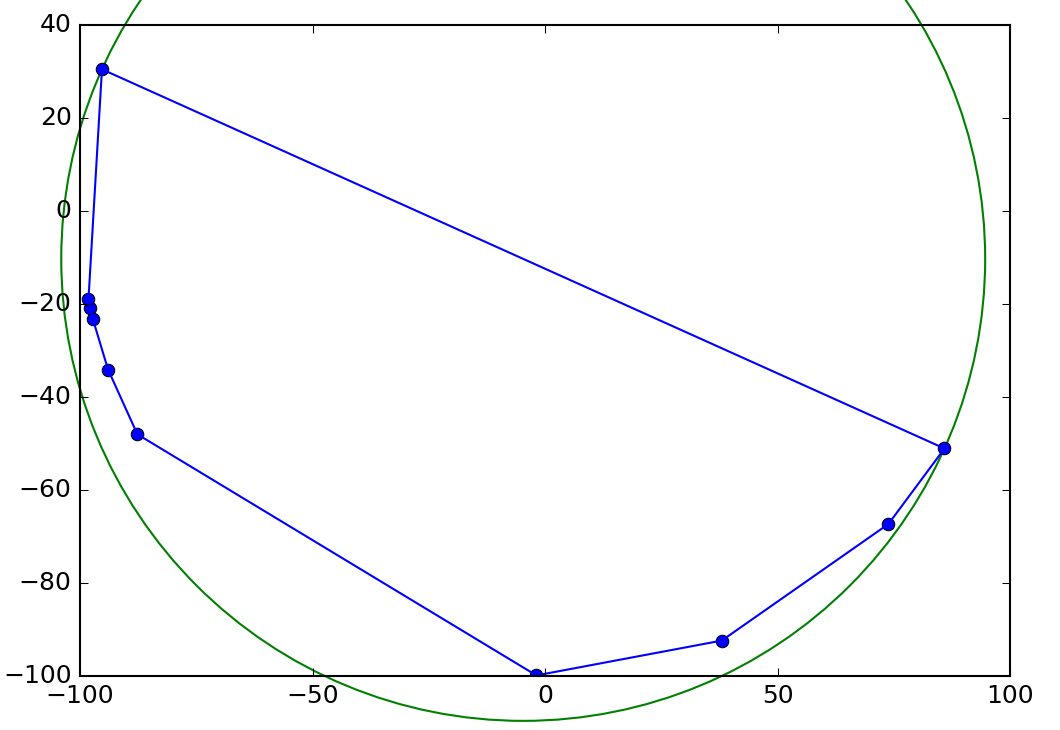
\includegraphics[width=0.7\textwidth]{pics/halfcircle/007.png}\\ ~ \\
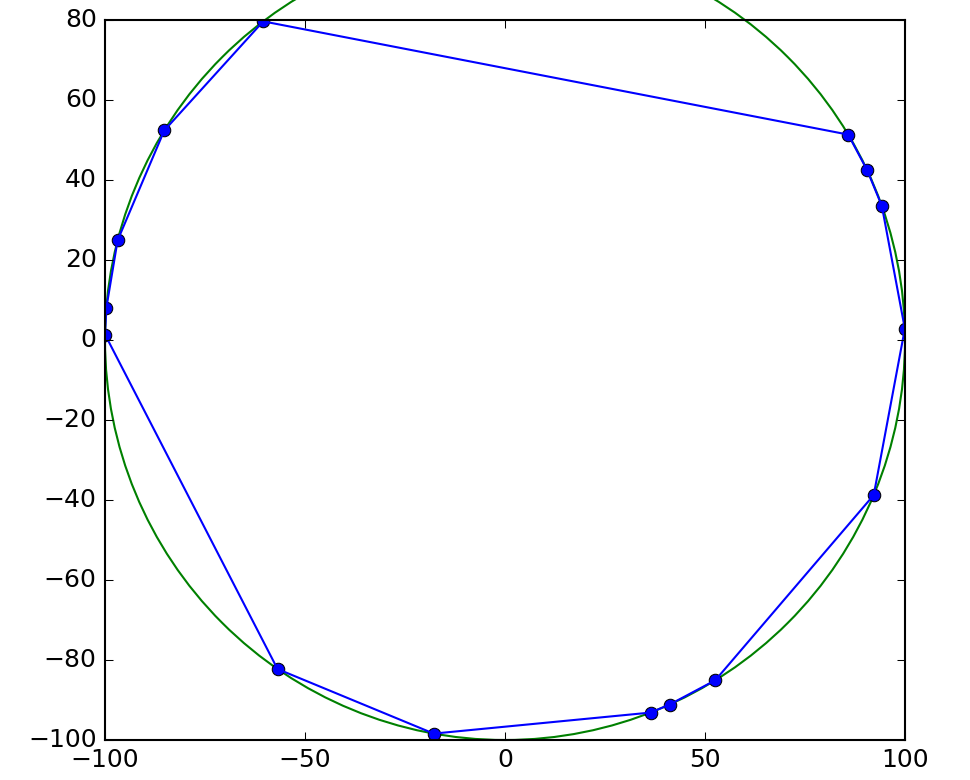
\includegraphics[width=0.7\textwidth]{pics/circle/005.png}
\end{center}

\newpage

\section{Wyszukiwanie najmniejszego prostokąta}

\subsection{Obserwacja}

Najmniejszy prostokąt można definiować jako prostokąt o najmniejszym obwodzie lub jako prostokąt o najmniejszym polu. Nie zawsze (choć dość często) będą to te same prostokąty: \\

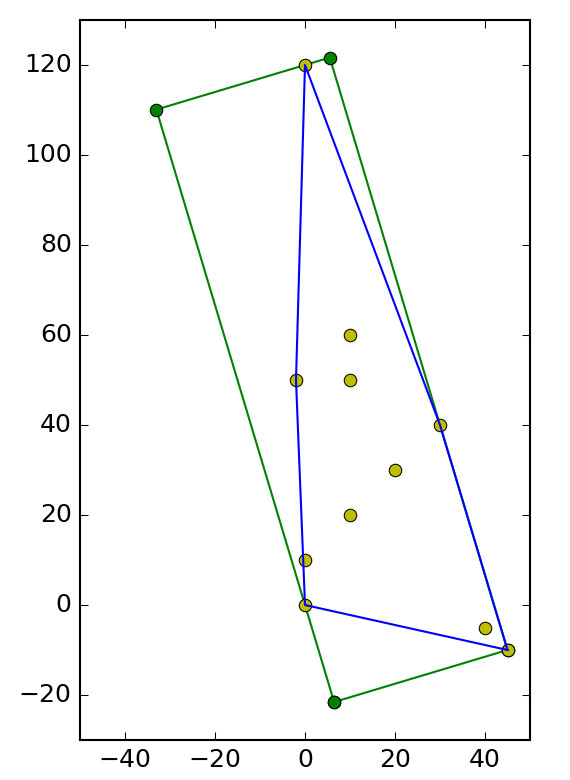
\includegraphics[width=0.5\textwidth]{pics/area.png}
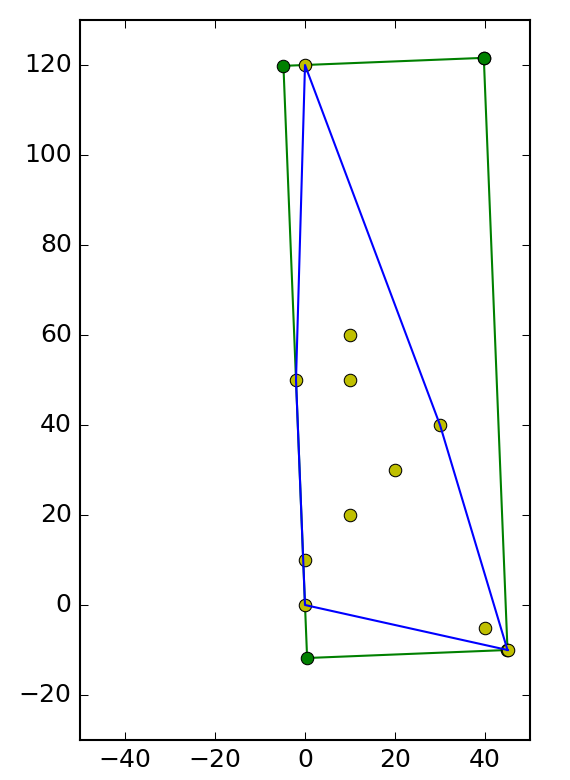
\includegraphics[width=0.5\textwidth]{pics/perim.png}
\newline \\
Powyżej po lewej znajduje się prostokąt o najmniejszym polu na tej chmurze punktów, po prawej o najmniejszym obwodzie na tej samej chmurze.

\newpage

\subsection{Wyszukiwanie najmniejszego prostokąta - pseudokod}

Powtarzaj dla każdej krawędzi otoczki:
\begin{enumerate}
\item „Obróć” otoczką, „kładąc” ją na kolejnej krawędzi na osi OX.
\item Oblicz pole i obwód prostokąta utworzonego przez skrajne punkty (z największą i najmnięjszą współrzędną x i y)
\item Zapamiętaj, który prostokąty był najmniejszy.
\end{enumerate}

\subsection{Wyszukiwanie najmniejszego prostokąta - implementacja}
Na kolejnej stronie znajduje się listing metody $run$ w klasie $Rectangle$ implementującej algorytm wyszukiwania najmniejszego prostokąta.

\newgeometry{margin=2cm}
Implementacja algorytmu znajdowania najmniejszego prostokąta:
\begin{center}
\lstinputlisting[language=Python,frame=single,linewidth=1\textwidth]{sourcecodes/rectangle.py}
\end{center}

\restoregeometry


\section{Obsługa programu}
\subsection{Wymagania}
Program napisany jest w języku Python 2.7. \\
Do uruchomienia programu potrzebna jest biblioteka $matplotlib$.

\subsection{Uruchomienie}
Repozytorium z kodem znajduje się pod adresem \url{https://github.com/jakubste/geo-project}. Można je stamtąd pobrać jako archiwum i wypakować na swoim komputerze lub sklonować używając Gita. \\ ~ \\
Każdy z algorytmów można zobaczyć urachamiając skrypty
\begin{lstlisting}[language=bash,frame=single,linewidth=1\textwidth]
$ python applet.py
$ python rectangle.py
\end{lstlisting}
~ \\ ~ \\
Nic nie stoi również na przeszkodzie, żeby użyć algorytmów w innym programie, importując odpowiednie klasy w swoim projekcie. Prawdopodobnie będzie przy tym konieczne usunięcie z działania programu zapisywania poszczególnych kroków programu jako obrazków oraz dostosowanie zwracanych przez program wartości.

\begin{lstlisting}[language=python,frame=single,linewidth=1\textwidth]
from applet import Applet


Applet(hull, points).run()
\end{lstlisting}

\begin{lstlisting}[language=python,frame=single,linewidth=1\textwidth]
from rectangle import SmallestRectangle


SmallestRectangle(hull, points).run('area')
SmallestRectangle(hull, points).run('perimeter')
\end{lstlisting}

\newpage

\subsection{Struktura repozytorium}

Poszczególne pliki lub katalogi zawierają:
\begin{itemize}
\item appet.py – Algorytm Appleta,
\item rectangle.py – algorytm wyznaczania najmniejszego prostokąta,
\item hull.py – dostarczony algorytm Grahama do wyznaczania otoczki wypukłej,
\item points\_generator.py – różne generatory losowych punktów,
\item prezentacja/ – prezentację z zajęć wraz z przykładem działania programu (obrazkami wygenerowanymi przez program),
\item dokumentacja/ – niniejszy dokument.
\end{itemize}

\subsection{Licencja}
Projekt udostępniony jest publicznie na warunkach licencji GNU General Public
Licence v.3.

\section{Bibliografia}
\begin{itemize}
\item Bartosz Sądel – Wyznaczanie minimalnego okręgu i prostokąta zawierającego chmurę punktów 2D \\
\url{https://prezi.com/ehey3lpea0dy/wyznaczanie-minimalnego-okregu-i-prostokata-zawierajacego-ch/}

\end{itemize}

\end{document}
